\documentclass[a4paper,12pt]{article}
\usepackage[utf8x]{inputenc}
\usepackage[czech, english]{babel}
\selectlanguage{english}
\usepackage[FM, EN, bwtitles, noheader]{tul}
\usepackage{hyperref}
\usepackage{float}
\usepackage{graphicx}
\usepackage{todonotes}
\presetkeys{todonotes}{inline}{}
\newcommand{\classname}[1]{\texttt{#1}}
\TULphone{+420\,485\,353\,030}
\TULmail{Petr.Jecmen@tul.cz}
\date{September 13, 2013}

\usepackage{listings}
\definecolor{gray}{rgb}{0.4,0.4,0.4}
\definecolor{darkblue}{rgb}{0.0,0.0,0.6}
\definecolor{cyan}{rgb}{0.0,0.6,0.6}
\lstset{
	basicstyle=\ttfamily,
	breaklines=true,
	keywordstyle=\color{darkblue},
	commentstyle=\color{gray},
    frame=trbl,
    rulecolor=\color{black!30},
    xrightmargin=7pt,
	columns=fullflexible,
	showstringspaces=false,
	language=Java
}
\lstdefinelanguage{XML}
{
	morestring=[b]",
	morestring=[s]{>}{<},
	morecomment=[s]{<?}{?>},
	identifierstyle=\color{darkblue},
	keywordstyle=\color{cyan},
	morekeywords={xmlns,version,type}
}

\begin{document}
\listoftodos
\newpage
\logo
\\\vspace{6pt}
\begin{center}
\large{\bfseries Manuál k softwaru GPU-DIC}
\\\vspace{1pc}
\small{
Ing. Petr Ječmen
\\\vspace{1pc}
Fakulta mechatroniky, informatiky a mezioborových studií\\
Technická Univerzita v~Liberci\\
Studentská 2\\
461 17 Liberec}
\end{center}
\newpage
\section{Úvod}
Algoritmus digitální obrazové korelace (dále jen DIC) se historicky ukázal jako algoritmus vhodný pro analýzu záznamu mechanických dějů pro potřeby analýzy chování materiálu s co největší přesností. Nevýhodou algoritmu je citlivost na vstupní parametry a dlouhá výpočetní doba. Cílem aplikace GPU-DIC je  hlavně zkrátit dobu výpočtu a alespoň částečný odhad vhodných vstupních parametrů.
Popis jak funguje algoritmus DIC lze nalézt v "Two-dimensional digital image correlation for in-plane displacement and strain measurement:a review, Bing Pan et al; 2009 Meas. Sci. Technol. 2;, http://iopscience.iop.org/0957-0233/20/6/062001." V tomto textu budou zmíněny pouze vybrané části, které byly vylepšeny nebo jejichž pochopením se uživateli ulehčí volba vstupních parametrů. V následující kapitole budou zmíněny pouze teoretické předpoklady pro úspěšnou volbu parametrů na základě teorie, detailnější doporučení týkající se volby parametrů budou pak uvedeny v kapitole \ref{sec:settings}.
\newpage
\section{Vybrané části algoritmu DIC}
V této části textu bude odkazováno na text uvedený v minulé kapitole, je tedy velmi doporučeno výše zmíněný text z webu stáhnout. Odkazy budou ve formě "(DIC-5)", kde číslovka označuje číslo strany.
\subsection{Dělba obrazu na facety}
Prvním krokem výpočtu je rozdělení obrazu na oblasti, v případě algoritmu jsou nazývány "facety" (ukázku lze nalézt v (DIC-5)). Výpočet probíhá nad jednotlivými facety a lze tušit, že volba velikosti a umístění facetu je klíčová pro úspěch algoritmu. Menší velikosti umožní zachycení detailů, zatímco větší pak nabízejí vetší odolnost proti šumu. V praxi se běžně používají velikosti okolo 15 pixelů, pro zašuměná videa pak není problém používat velikost 20 pixelů a více.
\subsection{Odhad deformace facetu}
Výpočet pole posunů tkví v odhadu, jak se facet deformoval. Facet se deformuje dle tzv. tvarové funkce, která popisuje možné varianty posunu jednotlivých pixelů ve facetu. Detailní popis funkce lze nalézt v (DIC-5). Hlavním parametrem tvarové funkce je řád funkce - nultý řád popisuje pouze posuny, první řád pak je schopen popsat protažení nebo zkosení, druhý řád už pak dokáže popsat i nelineární deformace. Nesmíme zapomenout, že daná funkce popisuje facet jako celek, nikoliv pixel po pixelu. To je výhodou a zároveň nevýhodou celého algoritmu. Výhodou je podobnost s realitou, kde se testované vzorky deformují opravdu jako celky, ne jako malinkaté pod-části. Nevýhodou je, že algoritmus je schopen otestovat pouze omezený počet variant deformací facetu a pokud řešení není v množině testovaných řešení, algoritmus nám předloží nějaké jiné řešení a není lehké stanovit, jestli je vybrané řešení opravdu to pravé nebo jen nejlepší ze skupiny zadaných. Řešením je předat algoritmu dostatečně velkou množinu možných deformací, to ale velmi prodlužuje dobu výpočtu, takže je nutné najít nějaký kompromis na základě předpokládaných deformací.
\subsection{Odhad pole přetvoření}
Výstupem algoritmu DIC je pole posunutí jednotlivých bodů (typicky bod = pixel). Pro potřeby mechaniky by bylo dobré kromě samotným posunů znát i pole přetvoření (hodnoty epsilon). Hodnota přetvoření je dána poměrem koncové délky ku počáteční, v diskrétní oblasti lze tedy definovat jako rozdíl hodnot posunů v daném směru (prostá diferenciace hodnot). Bohužel vlivem šumu nelze provést výpočet takto jednoduše. Existují dva přístupy, které dokáží potlačit vliv šumu na výsledné pole. Prvním přístupem je vyhlazení pole posunutí před vlastní diferenciací. Problém tohoto přístupu je volba vhodného vyhlazovacího algoritmu, který by nepotlačil užitečná data. Druhým přístupem a zároveň přístupem, který je implementován v aplikaci, je využití metody nejmenších čtverců. Podrobný popis lze nalézt v "Digital image correlation using iterative least squares and pointwise least squares for displacement field and strain field measurements. Bing Pan, Anand Asundi, Huimin Xie, Jianxin Gao. 2008." Principem metody je aproximace pole posunutí za pomoci lineární plochy (její předpis lze nalézt ve zmíněném článku) a hledání jejích koeficientů. Vzhledem k přímé závislosti koeficientů rovnice a hodnot posunutí a přetvoření, je možno koeficienty hledat za pomoci lineární algebry. Problém této metody je opět nutná volba parametru. Tím je velikost okolí, ve kterém se bude pole deformací aproximovat plochou. Pokud předpokládáme homogenní deformace, je možno volit velikost okna větší, protože se lépe potlačí vliv šumu ne přesnost výsledku. V případě velkých variací v poli posunutí je nutné volit menší okno, aby byly zachyceny detaily, a tím pádem může docházet ke zkreslení výsledků vlivem šumu. Typicky se velikost okna volí v rozsahu 11 - 21 pixelů.
\newpage
\section{Kroky výpočtu}
V této kapitole budou zmíněny kroky, které by měl uživatel vykonat před spuštěním vlastního výpočtu. Nastavení lze provést buď za pomoci grafického rozhraní (viz kapitola \ref{sec:gui}) nebo lze parametry také nastavit za pomoci skriptu úlohy (viz kapitola \ref{sec:config}).
\subsection{Vyznačení oblasti zájmu (ROI)}
Vzhledem k zaměření této aplikace na analýzu trhací zkoušky je i výpočet tomu uzpůsoben. Typicky záznam obsahuje region, kde je zkoušený předmět uchycen do čelistí a zbytek obrazu je pro analýzu nezajímavý. Proto uživatel může buď vyznačit obdélníkovou oblast(-i), na jejichž ploše bude probíhat výpočet, nebo využije možnosti dynamické tvorby ROI na základě polohy čelistí. V případě dynamické tvorby je nutno vyznačit úvodní polohu čelistí za pomoci kružnic, program poté sleduje polohu čelistí a upravuje oblast zájmu tak, aby byla mezi nimi.
\subsection{Vyznačení reálné velikosti}
Tento krok je volitelný a slouží k možné unifikaci velikosti plochy pro odhad plochy přetvoření. Aplikaci používá poměr px / mm, který lze opět zadat dvěma způsoby. Buď ve formě čísla do skriptu úlohy nebo za pomoci GUI, kde se vyznačí známý rozměr a jeho reálná velikost a poměr se automaticky dopočítá.
\subsection{Velikost facetu}
Velikost facetu je hlavním parametrem algoritmu a kvalita výsledky je na něm dost závislá. Doporučené hodnoty lze nalézt v kapitole \ref{sec:settings}. Číslo musí být celé a opět ho lze zadat přes GUI či skript.
\subsection{Expertní nastavení}
V některých speciálních případech může být žádoucí změnit i další parametry výpočetního enginu (jako limity deformací, limity kol výpočtu apod.). Co lze a nelze nastavit lze nalézt opět v kapitole \ref{sec:settings}, některá nastavení lze měnit v GUI, jiná se musí specifikovat za pomoci skriptu úlohy.
\newpage
\section{Ovládání aplikace}
\label{sec:gui}
\subsection{Úvodní okno}
\begin{figure}[H]
\center{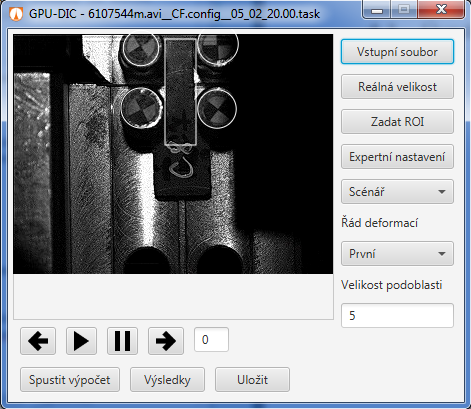
\includegraphics[width=0.5\textwidth]{hlavniOkno.png}\\Hlavní okno programu}
\end{figure}
\todo{screenshot okna, číselný popis prvků}
\subsection{Výběr vstupu}
\todo{video / obrázky / config / binary}
\subsection{Zadávání ROI}
\begin{figure}[H]
\center{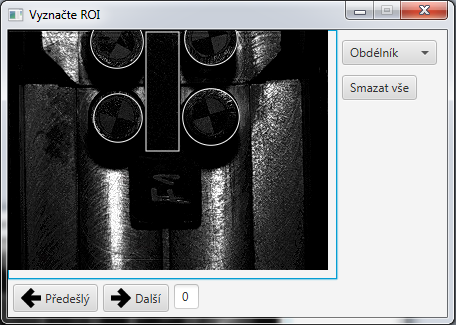
\includegraphics[width=0.5\textwidth]{ROI.png}\\Okno pro vyznačení ROI}
\end{figure}
\todo{jak se ovládá, jak se chová}
\subsection{Vyznačení reálné velikosti}
\begin{figure}[H]
\center{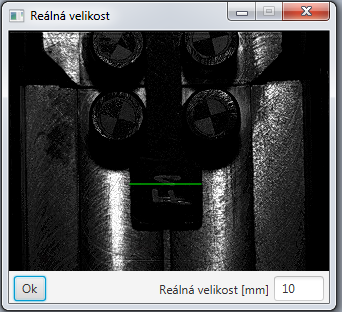
\includegraphics[width=0.5\textwidth]{realSize.png}\\Okno pro vyznačení reálné velikosti}
\end{figure}
\todo{jak se ovládá, jak se chová}
\subsection{Expertní nastavení}
\begin{figure}[H]
\center{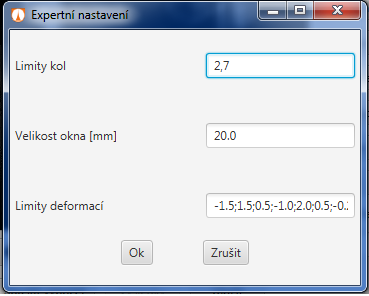
\includegraphics[width=0.5\textwidth]{expert.png}\\Expertní nastavení}
\end{figure}
\todo{odkaz na sekci s konfigurací úlohy}
\subsection{Spuštění výpočtu}
\todo{nic extra, pouze poznámka, že nenastavené parametry se nastaví na výchozí (uživatel se nemusí starat)}
\subsection{Uložení}
\begin{figure}[H]
\center{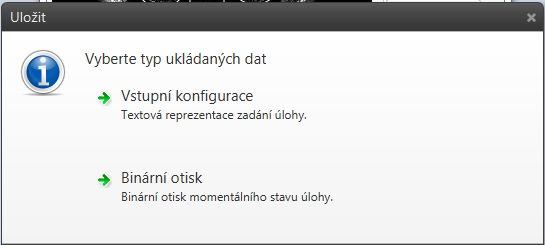
\includegraphics[width=0.5\textwidth]{saveCfgBin.png}\\Uložení projektu}
\end{figure}
\todo{uložení configu / bin. otisku}
\subsection{Výsledky}
\begin{figure}[H]
\center{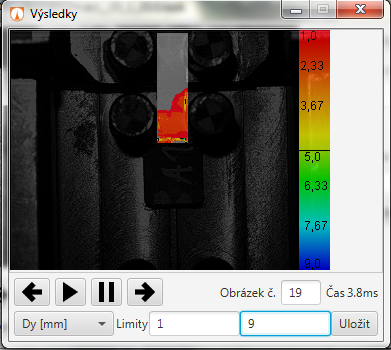
\includegraphics[width=0.5\textwidth]{results.png}\\Okno s výsledky}
\end{figure}
\todo{zobrazení výsledků a případné uložení}
\begin{figure}[H]
\center{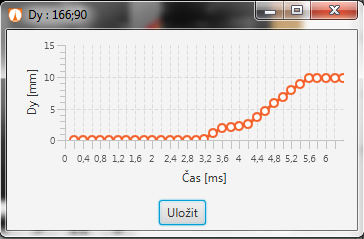
\includegraphics[width=0.5\textwidth]{resultsPoint.png}\\Výsledky pro bod}
\end{figure}

\newpage
\section{Konfigurační soubor úlohy}
\label{sec:config}
\todo{detailní popis možných položek v konfiguračním souboru}

\newpage
\section{Doporučená nastavení}
\label{sec:settings}
\todo{velikost facetu, parametr výpočtu přetvoření atd.}

% --- Zdrojove kody
\newpage
\todo{spravne zdrojove kody}
\section{Source code examples}
\subsection{Instance creation and messaging}\label{appMsg}
\begin{lstlisting}[title=Constant declaration]
final UUID ID = UUID.randomUUID();	// define ID for messaging
\end{lstlisting}
\begin{lstlisting}[title=Client side code]
public static void main(String[] args) {
  Client client = Client.Client.initNewClient();
  client.getListenerRegistrator().setIdListener(ID, new MessageHandler());
}

class MessageHandler implements Listener<Identifiable> {
  @Override
  public Object receiveData(Identifiable data) {
    if (data instanceof Message) {
      Message m = (Message) data;
      System.out.println(m.getData());	// print content to console
      return m.getHeader();	// send valid response
    } else {
      return "ERROR";	// report error
    }
  }
}
\end{lstlisting}

\subsection{Job Management}\label{appJm}
\begin{lstlisting}[title=Server side code]
public static void main(String[] args) {
  double start = -100.0, end = 100.0; // define range of values
  double step = 0.01;
  // divide the range in small pieces and create a Set<double[]>, where double[] defines start and end of each sub-range and step size
  for (double[] d : subranges) {	// submit all jobs
    s.getJobManager().submitJob(d);
  }
  s.getJobManager().waitForAllJobs();	// wait until all jobs are complete
  // use s.getJobManager().getAllJobs() to get all submitted jobs and find the best result
}

class DataStore implements DataStorage {
  @Override
  public Object requestData(Object o) {
    switch (o.toString()) {
      case "data":
        return dataArray;	// return data
      default:
        return "Illegal data request";
    }
  }
}
\end{lstlisting}

\end{document}